%%%%%%%%%%%%%%%%%%%%%%%%%%%%%%%%%%%%%%%%%%%%%%%%%%%%%%%%
%                       Assignment 2                   %
%                                                      %
% Author: Michael P. J. Camilleri					   %
%                                                      %
% Based on the Cleese Assignment Template for Students %
% from http://www.LaTeXTemplates.com.				   %
%                                                      %
% Original Author: Vel (vel@LaTeXTemplates.com)		   %
%													   %
% License:											   %
% CC BY-NC-SA 3.0 									   %
% (http://creativecommons.org/licenses/by-nc-sa/3.0/)  %
% 													   %
%%%%%%%%%%%%%%%%%%%%%%%%%%%%%%%%%%%%%%%%%%%%%%%%%%%%%%%%

%--------------------------------------------------------
%   IMPORTANT: Do not touch anything in this part
\documentclass[12pt]{article}
%%%%%%%%%%%%%%%%%%%%%%%%%%%%%%%%%%%%%%%%%
% Cleese Assignment
% Structure Specification File
% Version 1.0 (27/5/2018)
%
% This template originates from:
% http://www.LaTeXTemplates.com
%
% Author:
% Vel (vel@LaTeXTemplates.com)
%
% License:
% CC BY-NC-SA 3.0 (http://creativecommons.org/licenses/by-nc-sa/3.0/)
% 
%%%%%%%%%%%%%%%%%%%%%%%%%%%%%%%%%%%%%%%%%

%----------------------------------------------------------------------------------------
%	PACKAGES AND OTHER DOCUMENT CONFIGURATIONS
%----------------------------------------------------------------------------------------

\usepackage{lastpage} % Required to determine the last page number for the footer
\usepackage{graphicx} % Required to insert images
\setlength\parindent{0pt} % Removes all indentation from paragraphs
\usepackage[most]{tcolorbox} % Required for boxes that split across pages
\usepackage{booktabs} % Required for better horizontal rules in tables
\usepackage{listings} % Required for insertion of code
\usepackage{etoolbox} % Required for if statements
\usepackage{geometry} % Required for adjusting page dimensions and margins
\usepackage[utf8]{inputenc} % Required for inputting international characters
\usepackage[T1]{fontenc} % Output font encoding for international characters
\usepackage{fancyhdr} % Required for customising headers and footers
\usepackage{xspace}
\usepackage{booktabs}
\usepackage[colorlinks]{hyperref}
\usepackage{etoolbox}

\newcommand{\ie}{i.e.\@\xspace}
\newcommand{\eg}{e.g.\@\xspace}
\newcommand{\notemark}[1]{\textcolor{blue}{N.B.\ \emph{#1}}}
\newcommand{\noteself}[1]{\textcolor{red}{Thought: \emph{#1}}}
\newcommand{\note}[1]{\emph{\textbf{N.B.}\@\xspace#1}}
\newcommand{\hint}[1]{\emph{Hint: #1}}
\newcommand{\half}{$\frac{1}{2}$ }

\newbool{clearnext}		%Running Counter to see if clearing the page or not in the next subquestion.
\newbool{clearon}		%Parameter for specifying whether we will be clearing or not.
\newbool{authoron}		%Parameter to specify whether to show author or not

%----------------------------------------------------------------------------------------
%	Standard Template
%----------------------------------------------------------------------------------------
\geometry{
	paper=a4paper, % Change to letterpaper for US letter
	top=3cm, % Top margin
	bottom=3cm, % Bottom margin
	left=2.5cm, % Left margin
	right=2.5cm, % Right margin
	headheight=14pt, % Header height
	footskip=1.4cm, % Space from the bottom margin to the baseline of the footer
	headsep=1.2cm, % Space from the top margin to the baseline of the header
	%showframe, % Uncomment to show how the type block is set on the page
}
\pagestyle{fancy} % Enable custom headers and footers

%----------------------------------------------------------------------------------------
%	My Changes
%----------------------------------------------------------------------------------------
\lhead{\small\assignmentClass}
\chead{}
\ifbool{authoron}{\rhead{\small{\assignmentAuthorName}}}{\rhead{}}

\lfoot{} % Left footer
\cfoot{} % Centre footer
\rfoot{\small Page\ \thepage\ of\ \pageref{LastPage}} % Right footer

\renewcommand\headrulewidth{0.5pt} % Thickness of the header rule

%----------------------------------------------------------------------------------------
%	MODIFY SECTION STYLES
%----------------------------------------------------------------------------------------

\usepackage{titlesec} % Required for modifying sections

%------------------------------------------------
% Section

\titleformat
{\section} % Section type being modified
[block] % Shape type, can be: hang, block, display, runin, leftmargin, rightmargin, drop, wrap, frame
{\Large\bfseries} % Format of the whole section
{\assignmentQuestionName~\thesection} % Format of the section label
{6pt} % Space between the title and label
{} % Code before the label

\titlespacing{\section}{0pt}{0.5\baselineskip}{0.5\baselineskip} % Spacing around section titles, the order is: left, before and after

%------------------------------------------------
% Subsection

\titleformat
{\subsection} % Section type being modified
[block] % Shape type, can be: hang, block, display, runin, leftmargin, rightmargin, drop, wrap, frame
{} % Format of the whole section
{[\arabic{section}.\arabic{subsection}]} % Format of the section label (\alph{subsection})
{4pt} % Space between the title and label
{} % Code before the label

\titlespacing{\subsection}{0pt}{0.5\baselineskip}{0.5\baselineskip} % Spacing around section titles, the order is: left, before and after

\renewcommand\thesubsection{(\alph{subsection})}

%----------------------------------------------------------------------------------------
%	CUSTOM QUESTION COMMANDS/ENVIRONMENTS
%----------------------------------------------------------------------------------------

% Environment to be used for each question in the assignment
\newenvironment{question}[1]{
	\ifbool{clearon}{\clearpage}{}
	\global\setbool{clearnext}{false}
	\vspace{0.5\baselineskip} % Whitespace before the question
	\section{: #1}
	\lfoot{\small\itshape\assignmentQuestionName~\thesection~continued on next page\ldots} % Set the left footer to state the question continues on the next page, this is reset to nothing if it doesn't (below)
}{
	\lfoot{} % Reset the left footer to nothing if the current question does not continue on the next page
}

%------------------------------------------------

% Environment for inter-subquestion texts (no arguments)
\newenvironment{interquestiontext}{
	\ifbool{clearon}{\ifbool{clearnext}{\clearpage}{}}{}
	\global\setbool{clearnext}{false}
}{
}

%------------------------------------------------


%------------------------------------------------

% Environment for subquestions, takes 1 argument - the name of the section
\newenvironment{subquestion}[1]{
	\ifbool{clearon}{\ifbool{clearnext}{\clearpage}{}}{}
	\global\setbool{clearnext}{true}
	\subsection{#1}
}{
}

%------------------------------------------------

% Command to print a question sentence
\newcommand{\questiontext}[1]{
	\textbf{#1}
	\vspace{0.5\baselineskip} % Whitespace afterwards
	\global\setbool{clearnext}{false}
}

%------------------------------------------------
% Command to print a  Marking Scheme box.
\newcommand{\marking}[1]{
	\begin{tcolorbox}[colback=green!5!white,enhanced]
		\textbf{Marking Scheme:}#1
	\end{tcolorbox}
}

%------------------------------------------------

% Command to print a box that breaks across pages with the space for a student to answer
\newcommand{\model}[1]{
	\begin{tcolorbox}[enhanced]
		\textbf{Model Answer}:#1
	\end{tcolorbox}
}

\newcommand{\answerbox}[2]{
	\begin{tcolorbox}[enhanced, height=#1]
		#2
	\end{tcolorbox}
}

%------------------------------------------------

% Command to print an assignment section title to split an assignment into major parts
\newcommand{\assignmentSection}[1]{
	{
		\centering % Centre the section title
		\vspace{2\baselineskip} % Whitespace before the entire section title
		
		\rule{0.8\textwidth}{0.5pt} % Horizontal rule
		
		\vspace{0.75\baselineskip} % Whitespace before the section title
		{\LARGE \MakeUppercase{#1}} % Section title, forced to be uppercase
		
		\rule{0.8\textwidth}{0.5pt} % Horizontal rule
		
		\vspace{\baselineskip} % Whitespace after the entire section title
	}
}

%----------------------------------------------------------------------------------------
%	TITLE PAGE
%----------------------------------------------------------------------------------------

\title{
	\thispagestyle{empty} 		% Suppress headers and footers
	\vspace{0.01\textheight} 	% Whitespace before the title
	\textbf{\assignmentClass:\\ \assignmentTitle}\\[4pt]
	\ifbool{authoron}{\assignmentAuthorName}{
	\ifdef{\assignmentDueDate}{{\small Due\ on\ \assignmentDueDate}\\}{}
	{\large \textit{\assignmentWarning}}
	\vspace{0.01\textheight}} % Whitespace before the author name
}

\ifbool{authoron}{\author{Student: \textbf{\assignmentAuthorName}}}{}
\date{} % Don't use the default title page date field





% Options for Formatting Output

\global\setbool{clearon}{true} %
\global\setbool{authoron}{true} %



\newcommand{\assignmentQuestionName}{Question}
\newcommand{\assignmentTitle}{Assignment\ \#2}

\newcommand{\assignmentClass}{IAML -- INFR10069 (LEVEL 10)}

\newcommand{\assignmentWarning}{NO LATE SUBMISSIONS} % 
\newcommand{\assignmentDueDate}{Friday,\ November\ 15,\ 2019 @ 16:00}
%--------------------------------------------------------

%--------------------------------------------------------
%   IMPORTANT: Specify your Student ID below [You will need to uncomment the line, else compilation will fail]. Make sure to specify your student ID correctly, otherwise we may not be able to identify your work and you will be marked as missing.
\newcommand{\assignmentAuthorName}{s1709906}
%--------------------------------------------------------

\begin{document}
\maketitle
\thispagestyle{empty}



%%%%%%%%%%%%%%%%%%%%%%%%%%%%%%%%%%%%%%%%%%%%%%%%%%%%%%%%%%%%%%%%%%%%%%%%%%%%%%
%============================================================================%
%%%%%%%%%%%%%%%%%%%%%%%%%%%%%%%%%%%%%%%%%%%%%%%%%%%%%%%%%%%%%%%%%%%%%%%%%%%%%%


\assignmentSection{Part A: 20-NewsGroups [60 Points]}




\begin{question}{(10 points) Exploratory Analysis}

\questiontext{We will begin by exploring the Dataset to get some insight about it.}



\begin{subquestion}{(5 points) Focusing first on the training set, summarise the key features/observations in the data: focus on the dimensionality, data ranges, feature and class distribution and report anything out of the ordinary. What are the typical values of the features like?}


\answerbox{12em}{
The training set has 5866 entries, which means it has 5866 different documents, with 1001 unique words (key features). It also has 8 different class labels representing each news group. After grouping the data into their respective classes, I found out that out of all the newsgroups, class 7 (`soc.religion.christian`) has significantly fewer data compared to the other classes. All of the other classes have more than 700 values, but class 7 has lesser than 500. By examining the mean and standard deviation of each word, I could see that the words have similar low TF-IDF values.
}



\end{subquestion}


\begin{subquestion}{(3 points) Looking now at the Testing set, how does it compare with the Training Set (in terms of sizes and feature-distributions) and what could be the repurcussions of this?}


\answerbox{10em}{
The testing set has 1883 documents and 1001 unique words. The training set and the testing set are split 75\% - 25\%. This split is good because it does not overfit the model. There is a similar trend in the testing set with regards to the significantly lesser amount of data for class 7. All of the other classes have above 240 values and class 7 only has 157. The percentage of class 7 in the training set and the test set and they were both 8.34\%. This is not a problem in the test set, unlike the training set because it's never a good idea to train with lesser data for a certain class.
}



\end{subquestion}

\begin{subquestion}{(2 points) Why do you think it is useful to consider TF-IDF weights as opposed to just the frequency of times a word appears in a document as a feature?}



\answerbox{10em}{
TF-IDF weights is a statistical measure to evaluate how important a word is to a document in a collection. The importance of a word is directly proportional to the word frequency in the document, but it is offset by the frequency of the word in the entire collection.
It is useful to consider TF-IDF as opposed to just the word frequency in the document because it helps eliminate 'unimportant' words that are used frequently from the feature vectors by setting their weight close to 0, such as stop words. It also helps avoid irrelevant and costly computations.
}



\end{subquestion}



\end{question}


%============================================================================%

\begin{question}{\label{Q_UNSUP_LEARN}(24 points) Unsupervised Learning}

\questiontext{We will now explore the documents in some detail by way of clustering.}



\begin{subquestion}{(2 points) The K-Means algorithm is non-deterministic. Explain why this is, and how the final model is selected in the SKLearn implementation of \href{https://scikit-learn.org/stable/modules/clustering.html}{KMeans}.}



\answerbox{8em}{
Non-deterministic means that running the algorithm several times on the same data, could give different results (test points classified differently in each iteration). This is due to the algorithm's random selection of data points as initial cluster centres. In the SKLearn implementation of KMeans, we do not explicitly select the initial cluster centres - instead, the model will select them for us. This will speed up the convergence of the algorithm.
}



\end{subquestion}


\begin{subquestion}{(1 point) One of the parameters we need to specify when using k-means is the number of clusters. What is a reasonable number for this problem and why?}



\answerbox{5em}{
A reasonable number of clusters would be 8, because there are 8 news groups and we want to classify which words typically belong to which group.
}



\end{subquestion}


\begin{subquestion}{(5 points) We will use the Adjusted Mutual Information (AMI) \ie \href{https://scikit-learn.org/stable/modules/clustering.html\#mutual-info-score}{\texttt{adjusted\_mutual\\\_info\_score}} between the clusters and the true (known) labels to quantify the performance of the clustering. Give an expression for the MI in terms of entropy. In short, describe what the MI measures about two variables, why this is applicable here and why it might be difficult to use in practice. \hint{MI is sometimes referred to as Information Gain: note that you are asked only about the standard way we defined MI and not the AMI which is adjusted for the size of the domain and for chance agreement.}}



\answerbox{16em}{
The formula for Mutual Information (MI) in terms of entropy is the following:

\begin{equation} 
\text{MI}(U,V)= \sum_{i=1}^{|U|} \sum_{j=1}^{|V|} P(i,j)  \log{P(i,j)\over{P(i)P(j)}} = H(V) - H(V|U)
\end{equation}

where \textit{H(V)} is the entropy of \textit{V} and \textit{H(V|U)} is a measure of what \textit{V} doesn't say about \textit{U}. It follows that MI is the amount of information (decrease in uncertainty) you get about one variable given knowledge of another. MI calculates the statistical dependence between the two variables. Since words are not independent, knowing one of them can give us more information about the next word. MI based measures require the knowledge of the true class values which are almost never available in practice or require manual assignment by human annotators. 
}



\end{subquestion}

\begin{subquestion}{(4 points) Fit K-Means objects with \texttt{n\_clusters} ranging from 2 to 12. Set the random seed to 1000 and the number of initialisations to 50, but leave all other values at default. For each fit compute the adjusted mutual information (there is an SKLearn \href{https://scikit-learn.org/stable/modules/generated/sklearn.metrics.adjusted_mutual_info_score.html}{function} for that). Set \texttt{average\_method=`max'}. Plot the AMI scores against the number of clusters (as a line plot).}



\answerbox{40em}{
\begin{center}
    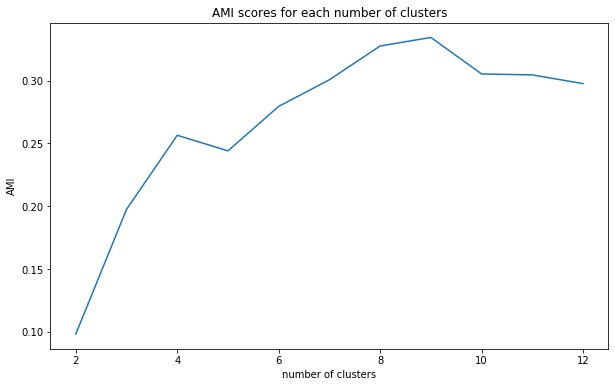
\includegraphics[width=0.9\textwidth]{2_d.png}
\end{center}
}



\end{subquestion}

\begin{subquestion}{(3 points) Discuss any trends and interesting aspects which emerge from the plot. Does this follow from your expectations?}



\answerbox{10em}{
The plot of AMI scores against the number of clusters shows a peak at n=9. I found this quite interesting because I expected that the AMI score will be the highest when there are 8 clusters, since there are 8 newsgroups. This might be because there are some ambiguous words that falls in more than 1 cluster and these ambiguous words are clustered together into a separate cluster, keeping the 8 other clusters relatively pure. As the number of clusters increase past 9, the AMI score decreases due to overfitting.
}



\end{subquestion}

\begin{subquestion}{\label{Q_CLUSTER_FOUR}(6 points) Let us investigate the case with four (4) clusters in some more detail. Using seaborn's \href{https://seaborn.pydata.org/generated/seaborn.countplot.html}{\texttt{countplot}} function, plot a bar-chart of the number of data-points with a particular class (encoded by colour) assigned to each cluster centre (encoded by position on the plot's x-axis). As part of the cluster labels, include the total number of data-points assigned to that cluster.}



\answerbox{40em}{
\begin{center}
    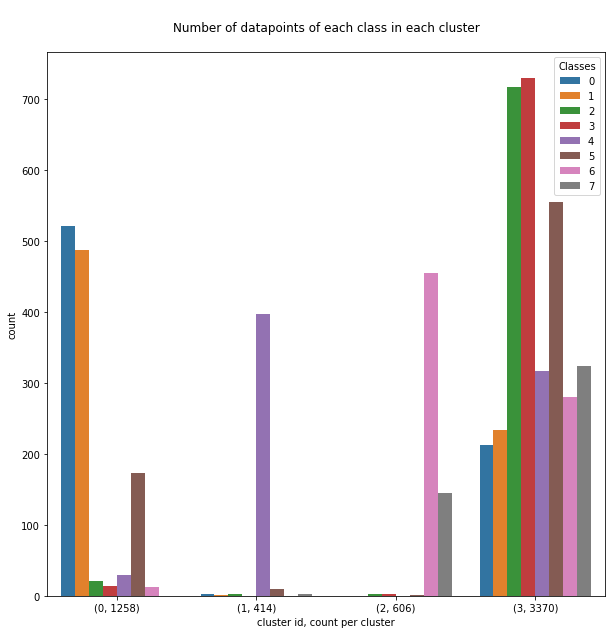
\includegraphics[width=0.9\textwidth]{2_f.png}
\end{center}
}



\end{subquestion}

\begin{subquestion}{(3 points) How does the clustering in Question\ref{Q_UNSUP_LEARN}:\ref{Q_CLUSTER_FOUR} align with the true class labels? Does it conform to your observations in Q 2(e)?}



\answerbox{14em}{
There are 4 bigger subgroups that you can generalise from the 8 newsgroups. This is noticeable in the bar chart - the 1st cluster has the main datapoint as classes 0, 1 and 5 (Electronics), the 2nd cluster contains almost only class 4 (Cryptography), the 3rd cluster has the classes 6 and 7 (Religion). The last cluster has a mix of all the classes but its main datapoint are classes 2 and 3 (Automotive).
The cryptography group is well-separated and this is well-identified by the clustering algorithm. The classes that are the hardest to determine by the cluster assignments are classes 2 and 3 which are confused with all the other classes. The plot conforms with my observations in Q(2.e) as there is a local maxima when the number of clusters is 4 and the clustering has been somewhat successful at separating the data into their bigger subgroups, however not all the clusters are pure.
}



\end{subquestion}



\end{question}

%============================================================================%

\begin{question}{(26 points) Logistic Regression Classification}
\label{Q_LR_NG}
\questiontext{We will now try out supervised classification on this data. We will focus on Logistic Regression and measure performance in terms of the \href{https://scikit-learn.org/stable/modules/generated/sklearn.metrics.f1_score.html}{F1} score (familiarise yourself with this score which is related to the precision and recall scores that we learnt about in class).}



\begin{subquestion}{(3 points) What is the F1-score, and why is it preferable to accuracy in our problem? How does the macro-average work to extend the score to multi-class classification?}



\answerbox{8em}{
The F1-score ((2*precision*recall)/(precision+recall)) conveys the balance between the precision and the recall. It is more preferable to use accuracy in our problem because false positives and false negatives have similar cost and we have relatively even classes. To calculate the classifier's overall F1-score combine the per-class F1-scores into a single number. The simplest way to do that is to is to compute an arithmetic mean of the per-class F1-scores, called the macro-average.
}



\end{subquestion}


\begin{subquestion}{(2 points) As always we start with a simple baseline classifier. Define such a classifier (indicating why you chose it) and report its performance on the \textbf{Test} set. Use the `macro' average for the \texttt{f1\_score}.} %\hint{For the baseline, the classifier should use only the target labels.}



\answerbox{8em}{
I selected the class that has the most observations (in this case it's a tie between classes 3 and 6) and used that class as the result for all the predictions. This method is theoretically expected to perform better than random guessing. 

After running the baseline classifier (predicting that all the values belong to class 3), I obtained the F1-score of 0.0292.
}



\end{subquestion}

\begin{subquestion}{(3 points) We will now train a \href{https://scikit-learn.org/stable/modules/generated/sklearn.linear_model.LogisticRegression.html}{LogisticRegression} Classifier from SKLearn. By referring to the documentation, explain how the Logistic Regression model can be applied to classify multi-class labels as in our case. \hint{Limit your explanation to methods we discussed in the lectures.}}



\answerbox{9em}{
The LogisticRegression Classifier can fit binary, One-vs-Rest, or multinomial logistic regression. Multi-class logistic regression utilises the softmax function to get the class probabilities. This function replaces the sigmoid logistic function used in binary logistic regression. The output of a softmax function is equal to the number of classes, and they sum up to one, therefore they are equal to the probabilities of each class.
}



\end{subquestion}

\begin{subquestion}{(4 points) Train a Logistic Regressor on the training data. Set \texttt{solver=`lbfgs'}, \texttt{multi\_class=`multinomial'} and \texttt{random\_state=0}. Use the Cross-Validation object you created and report the average validation-set F1-score as well as the standard deviation. Comment on the result.}



\answerbox{9em}{
Average validation-set F1-score = 0.668
\\Standard deviation = 0.0158
\\
\\The baseline classifier has significantly lower F1-score at 0.0291. Therefore, the logistic regression classifier performs significantly better than the baseline classifier. This shows a successful classification by the logistic model.
}



\end{subquestion}

\begin{subquestion}{\label{Q_LOG_REG_PLT}(5 points) We will now optimise the Regularisation parameter $C$ using cross-validation. Train a logistic regressor for different values of $C$: in each case, evaluate the F1 score on the training and validation portion of the fold. That is, for each value of $C$ you must provide the training set and validation-set scores per fold and then compute (and store) the average of both over all folds. Finally plot the (average) training and validation-set scores as a function of $C$. \hint{Use a logarithmic scale for $C$, spanning 19 samples between $10^{-4}$ to $10^5$.}}



\answerbox{40em}{
\begin{center}
    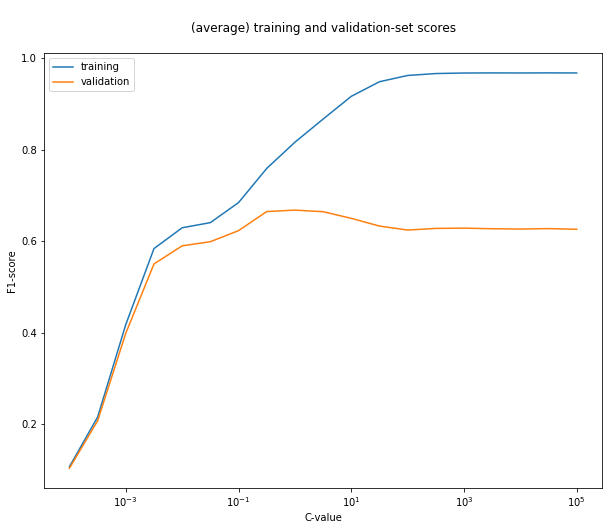
\includegraphics[width=0.9\textwidth]{3_e.png}
\end{center}
}



\end{subquestion}

\begin{subquestion}{(7 points) What is the optimal value of $C$ (and the corresponding score)? How did you choose this value? By making reference to the effect of the regularisation parameter $C$ on the optimisation, explain what is happening in your plot from Question \ref{Q_LR_NG}:\ref{Q_LOG_REG_PLT} \hint{Refer to the documentation for $C$ in the \href{https://scikit-learn.org/stable/modules/generated/sklearn.linear_model.LogisticRegression.html}{LogisticRegression} page on SKLearn}.}



\answerbox{11em}{
The most optimal value of C is 1.0 with a corresponding F1-score of 0.668. I chose this value by examining the F1-scores of the validation set and looked at the maximum, and find the corresponding value of C that yields that value. The effect of the regularisation parameter C on the optimisation is strong. This causes the model to become less sensitive to noise. However, at some point it becomes insensitive to important features. this is shown by the F1-score being low on small C values. Then the F1-score increases when C increased and reached its peak at 1.0, and after that it continues to decrease until it reaches a (somewhat) plateau.
}



\end{subquestion}

\begin{subquestion}{(2 points) Finally, report the score of the best model on the test-set, after retraining on the entire training set (that is drop the folds). \hint{You may need to set \texttt{max\_iter = 200}.} Comment briefly on the result.}



\answerbox{7em}{
The F1-score on the test set is 0.675 after using the optimal C-value and retraining on the entire training set. This value is higher than the average validation-set F1-score (0.668) that I calculated in Q(3.d) and the average validation-set F1-score (0.668) that I calculated in Q(3.e) using folds.
}



\end{subquestion}


\end{question}




%============================================================================%




%%%%%%%%%%%%%%%%%%%%%%%%%%%%%%%%%%%%%%%%%%%%%%%%%%%%%%%%%%%%%%%%%%%%%%%%%%%%%%
%============================================================================%
%%%%%%%%%%%%%%%%%%%%%%%%%%%%%%%%%%%%%%%%%%%%%%%%%%%%%%%%%%%%%%%%%%%%%%%%%%%%%%

\clearpage

\assignmentSection{Part B: Bristol Air-Quality [90 points]}




\begin{question}{\label{Q_EXPLORATORY}(30 Points) Exploratory Analysis}

\questiontext{We will begin by exploring the Dataset to familiarise ourselves with it.}



\begin{subquestion}{(6 points) Summarise the key features/observations in the data: describe the purpose of each column and report (briefly) also on the dimensionality/ranges (ballpark figures only, and how they compare across features) and number of sites, and identify anything out of the ordinary/problematic: \ie look out for missing data and negative values. Why are the latter unreasonable in such a dataset? \hint{Refer to the documentation for how to interpret the pollutant values.}}



\answerbox{13em}{
There are 1306758 values for each column - Date/Time, followed by the three pollutants, SiteID, and the latitude and longitude of the site. I observed that there are some samples that are either empty or have a value below 0 (negative), which is unreasonable because the values are measured in $\mu g/m^{3}$, and they only range over positive values. There are 18 unique sites in total that are being studied. Grouping the data into their respective SiteIDs, I noticed that there are significantly lesser values for site 15 than all the other sites, with only 2712 values, followed by site 0 with 6446. This is very few compared to sites 1, 5, 6, 7, 14, 16, which has more than 100000 values. All the other sites range between 10000 and 100000. For the pollutants, NOx has the highest mean, followed by NO and NO2.
}



\end{subquestion}

\begin{subquestion}{(6 points) Repeat the same analysis but this time on a per-site basis. Provide a table with the number of samples and percentage of problematic samples (negative and missing) in each site. To report numbers, count a row which has at least one missing entry
as having missing data, and similarly for negative entries. \hint{Pandas has a handy method, \texttt{to\_latex()}, for generating a latex table from a dataframe.}}



\answerbox{17em}{
\begin{adjustbox}
\small
\begin{tabular}{llllllllll}
\toprule
SiteID   &      0 &       1 &      2 &       3 &      4 &       5 &       6 &       7 &       8 \\
\midrule
Negative &      0 &       0 &      0 &   0.271 &      0 &       0 &       0 &       0 &       0 \\
Missing  &  1.613 &    6.29 &  4.348 &  77.333 &  2.069 &   8.828 &   7.444 &   4.195 &  21.057 \\
Total    &   6446 &  163111 &  62990 &   25464 &  74787 &  113952 &  142141 &  115162 &   43824 \\
\bottomrule
\end{tabular}
\\
\\
\begin{tabular}{llllllllll}
\toprule
SiteID   &      9 &     10 &     11 &      12 &      13 &      14 &    15 &      16 &     17 \\
\midrule
Negative &      0 &      0 &      0 &       0 &       0 &       0 &     0 &       0 &      0 \\
Missing  &  5.301 &   3.59 &  1.904 &  17.485 &  51.461 &  10.532 &   100 &   6.531 &  6.271 \\
Total    &  22071 &  96407 &  20693 &   45240 &   12423 &  113951 &  2712 &  154331 &  91053 \\
\bottomrule
\end{tabular}
\end{adjustbox}
\\
\\ * Negative and Missing values are in percentage (\%)}
\end{subquestion}

\begin{subquestion}{(4 points) Briefly summarise how the sites compare in terms of number of samples and amount of problematic samples.}



\answerbox{11em}{
Site 15 has the highest problematic values percentage of 100\%. After examining the table, I can see that there are no samples for site 15 (all the problematic values are due to missing samples). The next highest problematic values percentage belongs to Site 3 at 77.6\%, with a mixture of negative and missing samples. In fact, all the negative samples in the dataset belongs to Site 3. This value is followed by site 13 (51.46\%), site 8 (21.1\%), and site 12 (17.48\%). Every other site has a problematic sample percentage of less than 10\%.
}



\end{subquestion}

\begin{subquestion}{(3 points) Given that the columns are all oxides of nitrogen and hence we expect them to be related, we will now look at correlations in our data. This will also be useful in determining how well we can predict any one of the readings from the other two. Remove the data from sites 3 and 15 and compute the \textbf{Pearson} correlation coefficient between each of the three pollutant columns on the remaining data. Visualise the coefficients between each pair of columns in a table.}



\answerbox{10em}{
\newline   
\newline
\begin{tabular}{lrrr}
\toprule
{} &    NOx &    NO2 &     NO \\
\midrule
NOx &  1.000 &  0.878 &  0.988 \\
NO2 &  0.878 &  1.000 &  0.808 \\
NO  &  0.988 &  0.808 &  1.000 \\
\bottomrule
\end{tabular}
}



\end{subquestion}

\begin{subquestion}{(2 points) Comment on the level of correlation between each pair of pollutants.}



\answerbox{7em}{
The highest correlation is between NOx and NO, with a coefficient of 0.988. This is followed by the correlation of NOx and NO2, with a coefficient of 0.878. The lowest correlation is between NO2 and NO, with a coefficient of 0.808. Overall, I can observe that the pollutants have a strong positive correlation with each other.
}



\end{subquestion}



\begin{subquestion}{\label{CORRELATIONS}(5 points) For each of the three pollutants, compute the Pearson correlation between sites. \hint{You will need to remove the `Date Time' column and then group by the first level of the columns.} Then plot these as three heatmaps: show the values within the figures. \hint{Use the method \texttt{plot\_matrix()} from \texttt{mpctools.extensions.mplext}.}}



\answerbox{40em}{
\begin{center}
    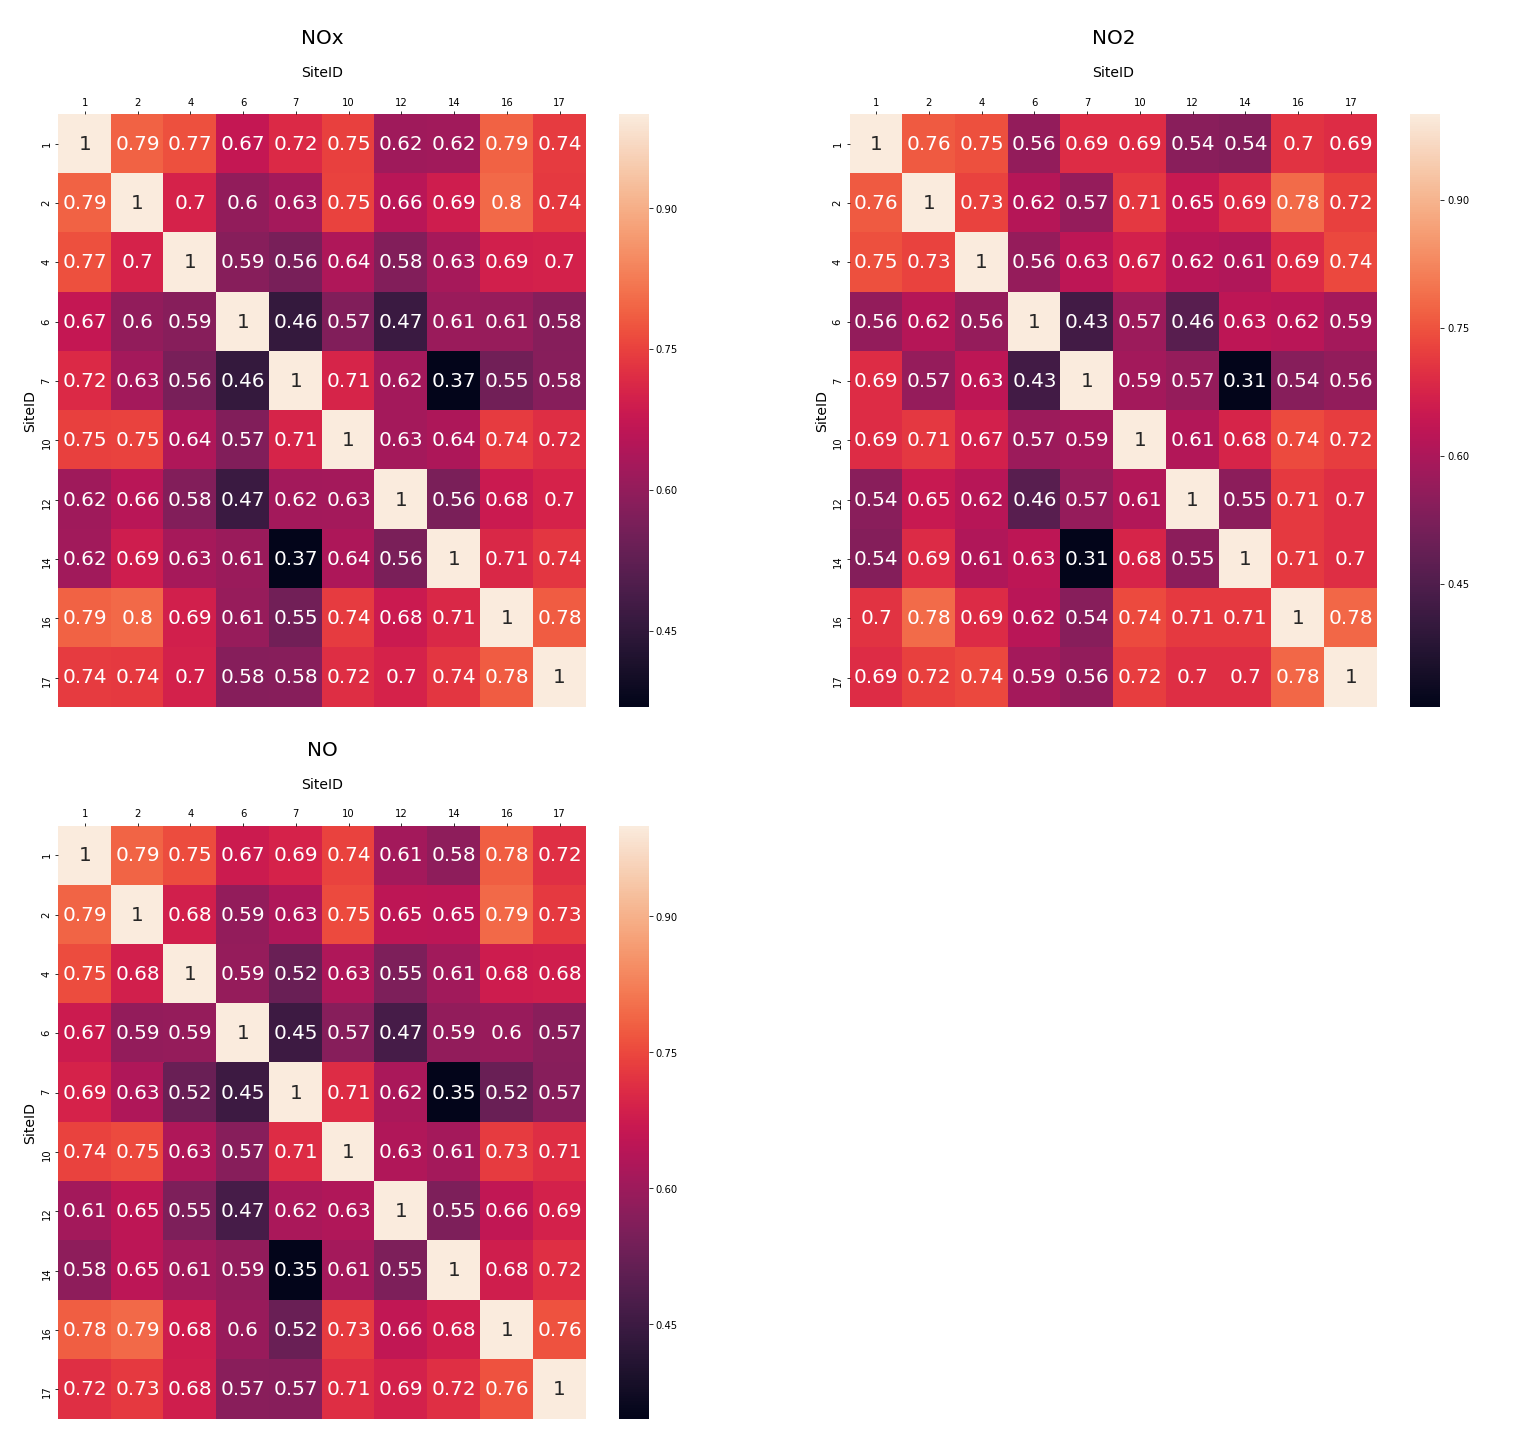
\includegraphics[width=1.0\textwidth]{4_f.png}
\end{center}
}



\end{subquestion}

\begin{subquestion}{(4 points) Comment briefly on your observations from Question \ref{Q_EXPLORATORY}:\ref{CORRELATIONS}: start by summarising the results from the NO gas and then comment on whether the same is observed in the other gases or if there is something different.}



\answerbox{12em}{
For NO gas, the highest correlation is between site 2 and 16 (0.79), followed by 1 and 16 (0.78), then 16 and 17 (0.76). The lowest correlation is between site 7 and 14 (0.35), followed by site 7 and 6 (0.45), then 6 and 12 (0.47). These trends are also spotted in NOx and NO2. In fact, the correlation between the sites for each pollutant varies very slightly, as the heatmap looks rather identical at first glance. The lowest correlation between sites can usually be found on NO2, and the highest correlation between sites can usually by found on NOx.
}



\end{subquestion}

\end{question}


%============================================================================%

\begin{question}{(19 Points) Principal Component Analysis}

\questiontext{One aspect which we have not yet explored is the temporal nature of the data. That is, we need to keep in mind that the readings have a temporal aspect to them which can provide some interesting insight. We will explore this next.}



\begin{subquestion}{(1 point) Plot the first 5 lines of data (plot each row as a single line-plot).}



\answerbox{40em}{
\begin{center}
    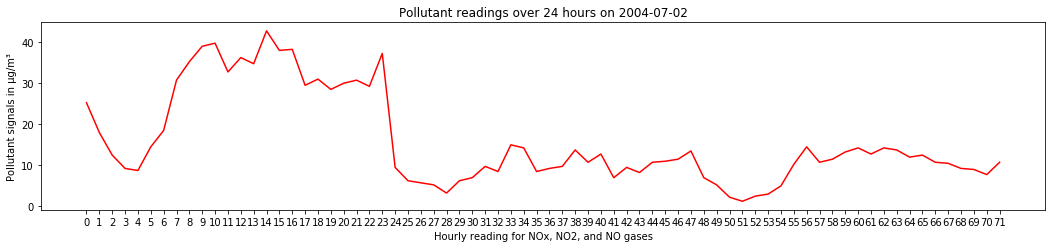
\includegraphics[width=0.9\textwidth]{5_a_1.png}
    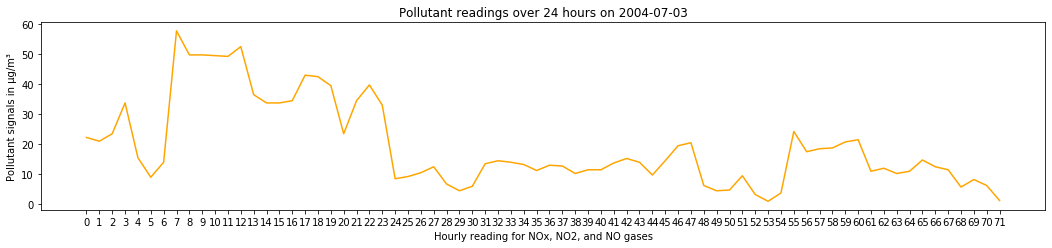
\includegraphics[width=0.9\textwidth]{5_a_2.png}
    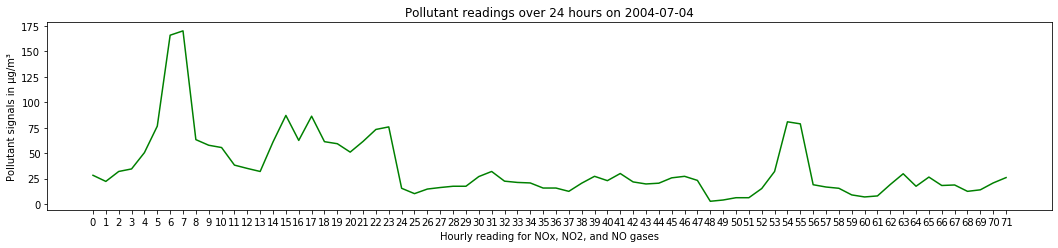
\includegraphics[width=0.9\textwidth]{5_a_3.png}
    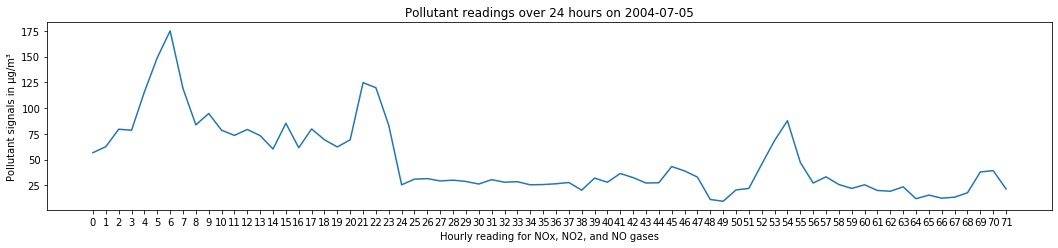
\includegraphics[width=0.9\textwidth]{5_a_4.png}
    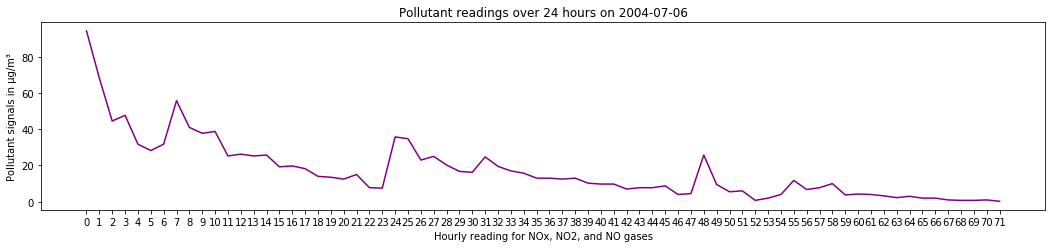
\includegraphics[width=0.9\textwidth]{5_a_5.png}
\end{center}
}



\end{subquestion}



\begin{subquestion}{(5 points) We will focus first on data solely from Site 1. Extract the data from this site, and run PCA with the number of components set to 72 for now. Set the \texttt{random\_state=0}. On a single graph plot: (i) the percentage of the variance explained by each principal component (as a bar-chart), (ii) the cumulative variance (line-plot) explained by the first $n$ components: (\hint{you should use \href{https://matplotlib.org/3.1.1/api/_as_gen/matplotlib.axes.Axes.twinx.html}{\texttt{twinx()}} to make the plot fit}), \textsl{and}, (iii) mark the point at which the number of components collectively explain at least 95\% of the variance (using a vertical line). \hint{Number components starting from 1.}}



\answerbox{40em}{
\begin{center}
    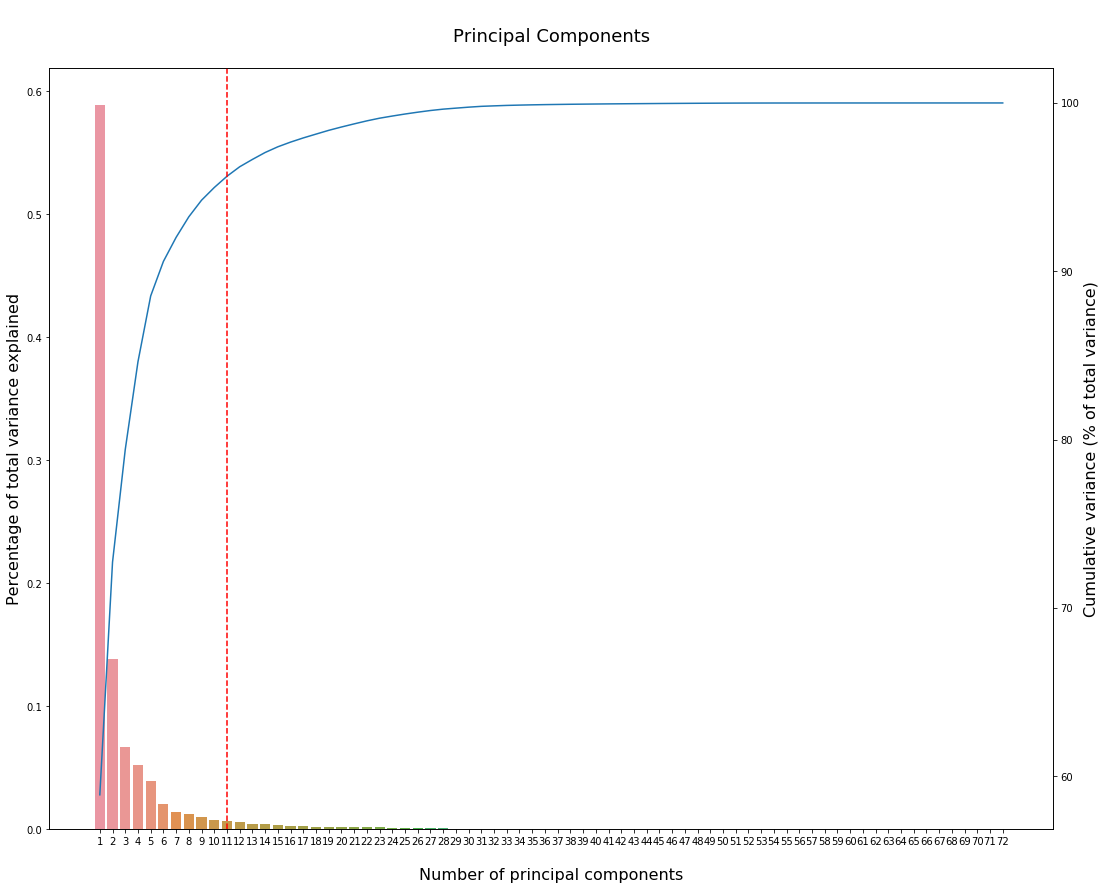
\includegraphics[width=1.0\textwidth]{5_b.png}
\end{center}
}



\end{subquestion}

\begin{subquestion}{(2 points) Interpret and summarise the above plot.}



\answerbox{9em}{
The percentage of total variance explained reduces exponentially as the number of principal components increase. The highest percentage of total variance explained is when the number of principal components is 1. The number of components which collectively explain at least 95\% of the variance is 10.
}



\end{subquestion}


\begin{subquestion}{(5 points) Generate three figures, one for the mean and one for each of the first 2 principal components: in each, plot the mean/component as three lines, one for each pollutant throught one day cycle. \hint{You will need to reshape the components appropriately.}}



\answerbox{50em}{
\begin{center}
    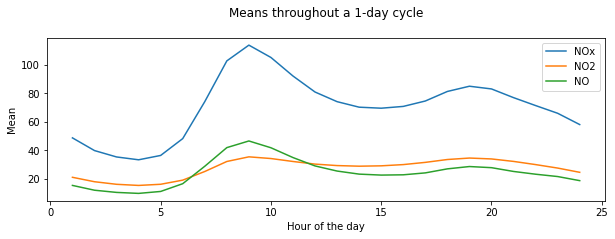
\includegraphics[width=1.0\textwidth]{5_d_mean.png}
    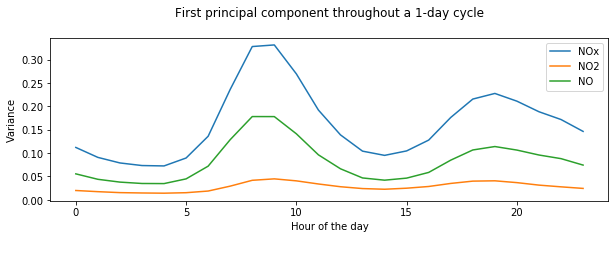
\includegraphics[width=1.0\textwidth]{5_d_pca1.png}
    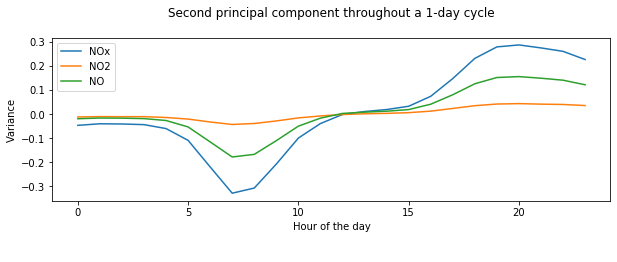
\includegraphics[width=1.0\textwidth]{5_d_pca2.png}
\end{center}
}



\end{subquestion}

\begin{subquestion}{(6 points) Focusing on the mean and first principal component, are there any significant patterns which emerge throughout the day? \hint{Think about car usage throughout the day.} What is different when interpreting the mean versus the first component? \hint{Do peaks signify the same thing in both cases?} Looking at the principal components only, are there any significant differences between the pollutants? Why could this be happening? \hint{You can refer to one of the limitations of PCA.}}



\answerbox{16em}{
For both the mean and first principal component, the general pattern is similar - pollutant levels are lowest at 4 AM, has a global maximum at 9 AM, reached a local minima at 3 PM and reaches a local maxima at 8 PM. This corresponds to the general car usage throughout the day, where people commute in the morning and come home in the evening. The highest pollutant value for both belongs to NOx. The peak in the mean shows the highest average measurement for a pollutant. The first principal component accounts for almost 60\% of the data and the peak signifies the highest variance amongst the 72 dimensions. The second component accounts for roughly 15\% of the variance of our data and has a much lower variance than the first principal component. This is as expected because the first principal component accounts for as much of the variability in the data as possible, and all the components after that accounts for as much of the remaining variability as possible.
}



\end{subquestion}

\end{question}

%============================================================================%


\begin{question}{\label{Q_LR_BA}(41 points) Regression}


\questiontext{Given our understanding of the correlation between signals and sites, we will now attempt to predict the NOx level for Site 17 given the value at the other sites. We will evaluate our models using the Root Mean Squared Error (RMSE) \ie the square root of the \href{https://scikit-learn.org/stable/modules/generated/sklearn.metrics.mean_squared_error.html}{mean\_squared\_error} score by sklearn.}



\begin{subquestion}{(2 points) First things first: since we are dealing with a supervised task, we will need to split our data into a training and testing set. Furthermore, since some of our regressors will involve hyper-parameter tuning, we will also need a validation set. Use the \texttt{multi\_way\_split()} method from \texttt{mpctools.extensions.skext} to split the data into a Training (60\%), Validation (15\%) and Testing (25\%) set: use the \href{https://scikit-learn.org/stable/modules/generated/sklearn.model_selection.ShuffleSplit.html}{ShuffleSplit} object from sklearn for the \texttt{splitter}. Set the random state to 0. \hint{The method gives you the indices of the split for each set, which can then be applied to multiple matrices.} Report the sizes of each dataset.}



\answerbox{4em}{
Training set: 8937, validation set: 2234, testing set: 3724
}



\end{subquestion}

\begin{subquestion}{(4 points) Let us start with a baseline. By using only the $y$-values, what baseline regressor can you define (indicate what it does)? Implement it and report the RMSE on the training and validation sets. Interpret this relative to the statistics of the data.}



\answerbox{8em}{
The baseline regressor that I used assigns the central tendency measure as the result for all predictions. The central tendency measure that I chose is the mean. 
\\
\\ The RMSE of the baseline regressor on the training set is: 79.714
\\ The RMSE value of the baseline regressor on the validation set is: 80.205
}



\end{subquestion}

\begin{subquestion}{(3 points) Let us now try a more interesting algorithm: specifically, we will start with \href{https://scikit-learn.org/stable/modules/generated/sklearn.linear_model.LinearRegression.html}{LinearRegression}. Train the regressor on the training data and report the RMSE on the training and validation set, and comment on the relative performance to the baseline.}



\answerbox{7em}{
\\The RMSE value for the training set is: 39.835
\\The RMSE value for the validation set is: 41.127
\\From these values we can observe that the Linear Regression algorithm does significantly better than the baseline regressor.
}



\end{subquestion}



\begin{subquestion}{(5 points) We want to explore further what the model is learning. Explain why in Linear Regression, we cannot just blindly use the weights of the regression coefficients to evaluate the relative importance of each feature, but rather we have to normalise the features. By referring to the documentation for the \href{http://scikit-learn.org/stable/modules/generated/sklearn.linear_model.LinearRegression.html}{LinearRegression} implementation in SKLearn, explain what the normalisation does and how it helps in comparing features. Will this affect the performance of the Linear Regressor?}



\answerbox{10em}{
The magnitude of the regression coefficient indicates how much a unit-change in the independent variable affects the target variable, therefore it depends on the magnitude of the independent and dependent variable to begin with. If the two attributes are not on the same scale, we have to normalize them so that we can compare them. When you set \texttt{normalize=True}, the regressor's X values will be normalized before regression. The values are normalized by subtracting the mean and dividing by the l2-norm.
}



\end{subquestion}

\begin{subquestion}{(5 points) Retrain the regressor, setting \texttt{normalize=True} and report (in a table) the ratio of the relative importance of each feature. Which is the most/least important site? How do they compare with the correlation coefficients for Site 17 as computed in Question \ref{Q_EXPLORATORY}:\ref{CORRELATIONS}, and why do you think that is?}



\answerbox{15em}{
\begin{tabular}{ll}
\begin{tabular}{rr}
\toprule
 SiteID &  Correlation Coefficient \\
\midrule
      6 &                -0.006799 \\
      2 &                 0.009947 \\
      7 &                 0.059388 \\
     10 &                 0.079779 \\
     14 &                 0.094507 \\
\bottomrule
\end{tabular}
&
\begin{tabular}{rr}
\toprule
 SiteID &  Correlation Coefficient \\
\midrule
      1 &                 0.115556 \\
     12 &                 0.129110 \\
      4 &                 0.134139 \\
     16 &                 0.161828 \\
\bottomrule
\end{tabular}
\end{tabular}
\\
\\The most important site is site 16 (0.162) and the least important site is site 6 (-0.007). These values correspond to the values computed in Q(4.f). This is because if the variable is strongly positively correlated to the target variable, it will have a big weight in linear regression, and affect the predicted value more.
}



\end{subquestion}

\begin{subquestion}{(5 points) It might be that with non-linear models, we may get better performance. Let us try to use \href{https://scikit-learn.org/stable/modules/generated/sklearn.neighbors.KNeighborsRegressor.html}{K-Nearest-Neighbours}. Train a KNN regressor with default parameters on the training set and report performance on the training and validation set. \hint{it might be beneficial to set \texttt{n\_jobs=-1} to improve performance.} How does it compare with Linear Regression in terms of performance on both sets? What is a limitation of the KNN algorithm for our dataset?}



\answerbox{8em}{

KNN regression RMSE on the training set: 32.437 | validation set: 40.307

Linear Regression RMSE on the training set: 39.835 | validation set: 41.127

From these values we can observe that the KNN regression performs better than linear regression. The limitation of the KNN algorithm on our dataset is that it is computationally costly to calculate the distance between a new point point and all the existing points, hence the performance of the algorithm degrades.
}



\end{subquestion}

\begin{subquestion}{(4 points) The KNN regression allows setting a number of hyper-parameters. We will optimise only one: the number of neighbours to use. By using the validation set, find the optimal value for the \texttt{n\_neighbours} parameter out of the values [2, 4, 8, 16, 32]. Plot the training/validation RMSE and indicate (for example with a line) the best value for \texttt{n\_neighbours}.}



\answerbox{40em}{
\begin{center}
    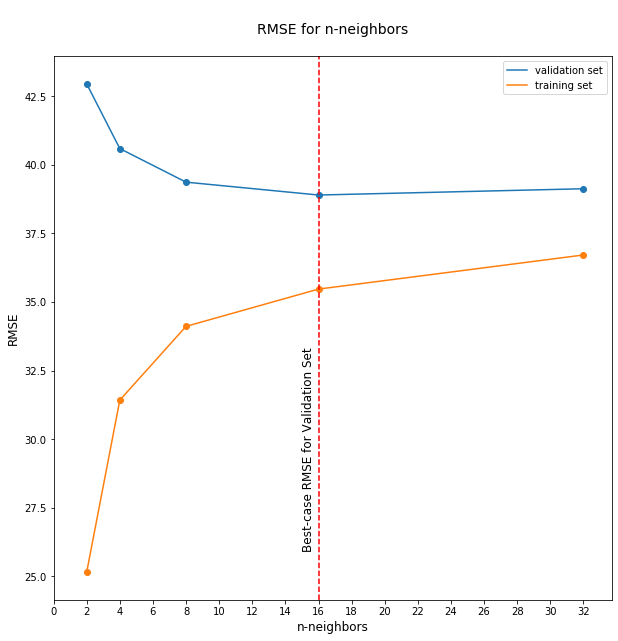
\includegraphics[width=0.9\textwidth]{6_g.png}
\end{center}
}



\end{subquestion}

\begin{subquestion}{(1 points) What is the best-case RMSE performance on the validation set for KNN?}



\answerbox{6em}{
The best-case RMSE performance on the validation set is 38.902. This is obtained when \texttt{n\_neighbors} is set to 16.
}



\end{subquestion}

\begin{subquestion}{(4 points) Let us try one last regression algorithm: we will now use \href{https://scikit-learn.org/stable/modules/generated/sklearn.tree.DecisionTreeRegressor.html}{DecisionTreeRegressor}. Again, the algorithm contains a number of hyper-parameters, and we will optimise the depth of the tree. Train a series of Decision Tree Regressors, optimising (over the validation set) the \texttt{max\_depth} over the values [2, 4, 8, 16, 32, 64]. Set \texttt{random\_state=0}. Plot the training/validation RMSE and indicate (as before) the best value for \texttt{max\_depth}.}



\answerbox{40em}{
\begin{center}
    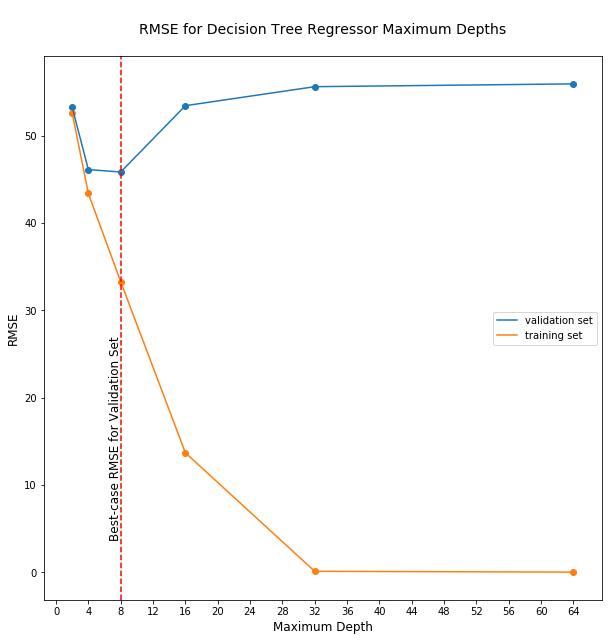
\includegraphics[width=0.9\textwidth]{6_i.png}
\end{center}
}



\end{subquestion}

\begin{subquestion}{(3 points) What is the best-case RMSE performance on the validation set? What do you notice from the plot about the performance of the Decision Tree Regressor?}



\answerbox{6em}{
The best-case RMSE on the validation set is 45.844, with a corresponding \texttt{max\_depth} value set at 8. For the training set, increasing max depth reduces the RMSE to zero. For the validation set, increasing max depth overfits the training data without capturing useful patterns and cause RMSE to increase.
}



\end{subquestion}

\begin{subquestion}{(5 points) To conclude let us now compare all the models on the testing set. Combine the training and validation sets and retrain the model from each family on it: in cases where we optimised hyper-parameters, set this to the best-case value. Report the testing-set performance of each model in a table \hint{You should have 4 values}.}



\answerbox{6em}{
\begin{tabular}{ll}
\begin{tabular}{lr}
\toprule
Regressor &  RMSE on Testing Set \\
\midrule
 Baseline &            78.952130 \\
   Linear &            40.509027 \\
\bottomrule
\end{tabular}
&
\begin{tabular}{lr}
\toprule
     Regressor &  RMSE on Testing Set \\
\midrule
           KNN &            37.984965 \\
 Decision Tree &            43.068871 \\
\bottomrule
\end{tabular}
\end{tabular}

}



\end{subquestion}

\end{question}

%============================================================================


\end{document}